\documentclass[acmsmall,screen,review,anonymous]{acmart}

%% ISSTA 2027 Research Papers: 18 pages incl. appendix,
%% excluding Data Availability and references.
%% Target: 36th ACM SIGSOFT International Symposium on Software Testing and
%% Analysis (ISSTA 2027), Singapore, 7-10 September 2027.
%% Abstract deadline 2027-01-08, full paper 2027-01-11, camera-ready 2027-07-22.

\usepackage{booktabs}
\usepackage{graphicx}
\usepackage{amsmath}
\usepackage{xspace}
\usepackage{multirow}

\newcommand{\sys}{\textsc{DeltaScope}\xspace}
\newcommand{\ie}{i.e.,\xspace}
\newcommand{\eg}{e.g.,\xspace}

% 浮动体参数：减少整页留白（5 图 7 表，单栏）
\setcounter{topnumber}{3}
\setcounter{bottomnumber}{2}
\setcounter{totalnumber}{6}
\renewcommand{\topfraction}{0.92}
\renewcommand{\bottomfraction}{0.5}
\renewcommand{\textfraction}{0.06}
\renewcommand{\floatpagefraction}{0.78}

\acmConference[ISSTA '27]{Proceedings of the 36th ACM SIGSOFT International Symposium on Software Testing and Analysis}{September 7--10, 2027}{Singapore, Singapore}
\acmBooktitle{Proceedings of the 36th ACM SIGSOFT International Symposium on Software Testing and Analysis (ISSTA '27)}
\acmYear{2027}
\copyrightyear{2027}

\begin{document}

\title{Compiling Auditable Licences from Change Orders:\\
A Work-Point Study of PLC Change Review}

\author{Anonymous Author(s)}
\affiliation{\institution{Anonymous Institution}\country{China}}

\begin{abstract}
PLC change review asks a question that compilation, type checking and simulation do not: \emph{should this edit have landed here at all?} Coding agents almost always make the requested change, but only 11--20\% of their edits match the scope the developer intended, and a single scan cycle of unintended output can move an actuator. Existing gates check whether the new code is legal; none checks whether the edit is within the scope the work order granted.

We compile the work order into an auditable licensed region---which outputs may change, under which operating condition, and for how long---and decide containment by cycle-accurate differential execution. On 96 PLC programs and 250 over-edit patches (246 observable) the procedure detects 92.3\% of cases whose boundary is statically expressible and 85.4\% corpus-wide, with zero false alarms in 272 controls, at 235\,ms per case and no API cost.

An 18-configuration study places this result on a short Pareto frontier: the method is the only zero-false-alarm point, while the strongest LLM judge reaches 100\% recall only at 5.5\% false alarms, and is the better choice solely when a missed over-edit costs more than $8.4\times$ a false alarm. The frontier position is set by contract tightness---activation rate and licensed-output width---not by the decision engine. Finally, rewriting only the wording of a work order moves the violation rate from 6/6 to 0/10 with byte-identical patches, making order clarity a larger lever than any detector we compared.
\end{abstract}

\maketitle

\section{Introduction}

\subsection{A change that compiles, type-checks, simulates---and is still wrong}

A packaging line needs one sentence changed: \emph{``start 2\,s after the emergency-stop reset.''} An agent edits the program in forty seconds. The code compiles, the type checker is silent, the closed-loop simulation passes. Three days later, under an overload condition, the motor does not stop in time: while editing the delay, the agent had also deleted an overload interlock it judged redundant.

We use this as a \textbf{composite scenario}, synthesised from prior work on agent edits and from our interviews with PLC maintenance engineers; it is illustrative, not an incident we observed. Its point is structural: \textbf{all three gates check whether the new code is legal, and none checks whether this edit should have landed here at all.}

The gap is not hypothetical. In a study of four coding agents on 387 real log-deletion tasks, edits were \emph{effective} in 95.6--100\% of cases but \emph{scope-consistent with the stated intent} in only 11.1--19.6\%. In PLC code that surplus is not a style issue: one scan cycle of unintended output can move an actuator, and passing compilation poorly predicts correct behaviour.

\subsection{What existing checks answer, and the question none of them asks}

Four families of tools are routinely applied to a PLC change, and each answers a different question:

\begin{table}[htbp]
\centering
\small
\begin{tabular}{@{}p{0.20\columnwidth}p{0.24\columnwidth}p{0.46\columnwidth}@{}}
\toprule
family & question answered & why it does not answer ours \\
\midrule
semantic-preservation diffing & \emph{did behaviour change?} & a licensed change also changes behaviour; a behavioural-equality test flags it by design \\
formal verification & \emph{is the new code correct w.r.t.\ a specification?} & the engine is reliable, but a human must first write the specification---and the specification of ``what this work order permits'' is exactly what is missing \\
static rule mining & \emph{does it match rules extracted from history?} & no execution, so timing- and window-shaped over-edits are invisible \\
asking a general model & \emph{does it look right?} & no boundary is defined, so the answer moves when the prompt does \\
\bottomrule
\end{tabular}
\caption{Four families of existing checks and the question they leave open.}
\label{tab:families}
\end{table}

The question in the gap is \textbf{``should this change have happened here?''} To our knowledge---we searched ACM DL, IEEE Xplore and arXiv in November 2026---no published work poses it as a task with an executable decision procedure.

\subsection{The task, and three deliberate choices}

We formalise it as a containment problem. Given a program $P$, a work order $C$ in natural language, and a candidate patch $P'$:

\begin{equation}
\mathrm{Diff}(P,P') \;\subseteq\; L(C)
\label{eq:containment}
\end{equation}

where $\mathrm{Diff}$ is the set of behavioural differences observed by executing both versions cycle by cycle on the same input distribution, and $L(C)$ is the \emph{licensed} region compiled from the order: which outputs may change, under which operating condition, and for how long. Three choices are deliberate and each has a cost we accept:

\begin{itemize}
\item \textbf{Behaviour, not text.} A refactoring that rewrites everything and changes nothing must be licensed; a one-token edit can still move an output.
\item \textbf{Containment, not equality.} Real changes almost always produce some difference; demanding equality would reject every correct patch.
\item \textbf{Output-level, conditioned, and bounded in magnitude.} Hitting the right output with the wrong magnitude (500\,ms $\to$ 3\,s) is still an over-edit, and a detector that ignores magnitude cannot say so.
\end{itemize}

\subsection{Results in one page}

We evaluated the method against 18 configurations on 96 programs and 522
cases: six formal\slash differential configurations, five static ones, six
general-model judges (three models $\times$ two prompts), plus one reference
arm. Three results frame the rest of the paper; Figure~\ref{fig:clarity} shows the first.

\begin{figure}[htbp]
\centering
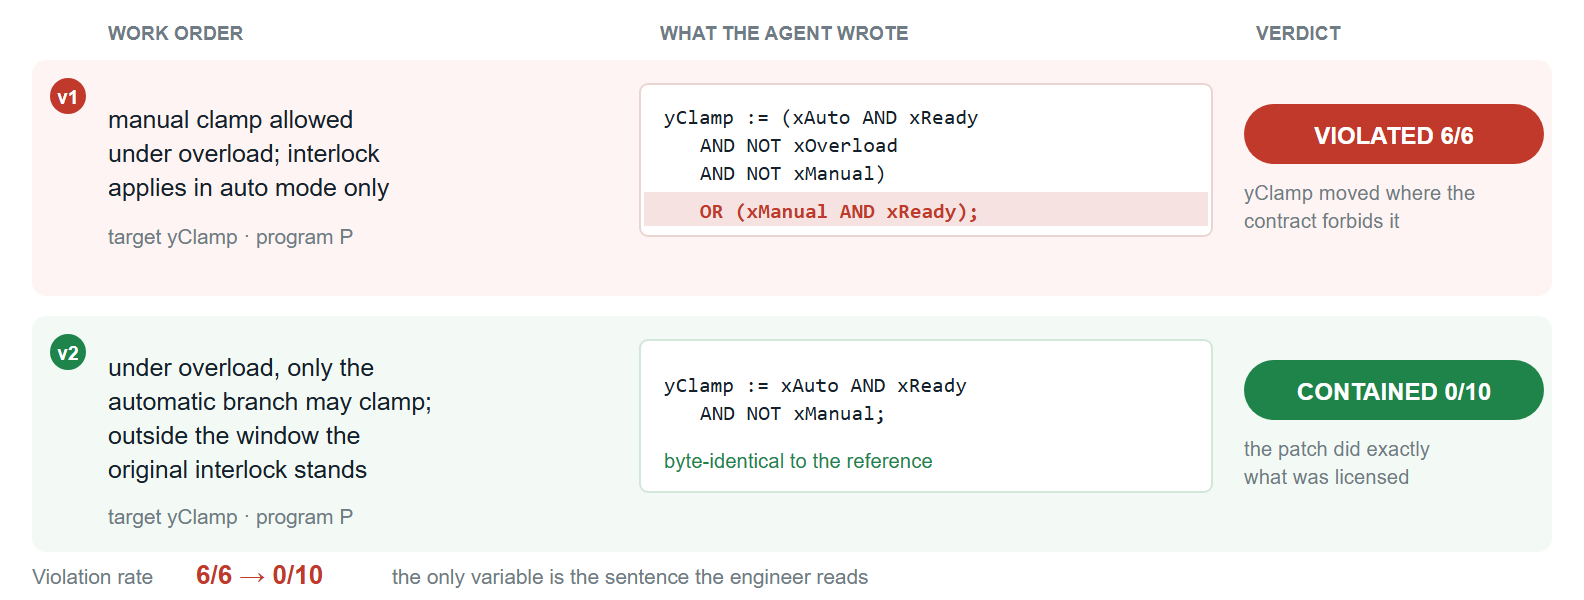
\includegraphics[width=\columnwidth]{figures/fig1.png}
\caption{One change, two ways to write the order. Program, model families and
the compiled contract are identical; only the sentence changes. \textbf{Top:}
the ambiguous order licenses manual clamping ``under overload'', so the agent
adds a bypass branch, and every patch (6/6) moves \texttt{yClamp} outside the
licensed guard. \textbf{Bottom:} once the order states that the manual branch is
unchanged and that the interlock stands outside the window, all ten patches are
byte-identical to the reference and none is flagged. Violation rate 6/6 $\to$
0/10 with nothing else changed.}
\label{fig:clarity}
\end{figure}

\textbf{The method is the zero-false-alarm point of a short frontier.}
It detects \textbf{85.4\%} of observable over-edits (210/246), and
\textbf{92.3\%} (155/168) on the statically expressible layer, with
\textbf{0/272 false alarms}. No configuration in the comparison achieves a
better recall at FPR $\le$ 1\%.

\textbf{On balanced accuracy, two baselines are better---and we say so.} A Qwen-based LLM judge reaches 97.0\% correct on the 506 pairable cases against our 92.9\% (Holm-corrected $p = 9.2\mathrm{e}{-03}$); the AI-contract arm reaches 96.8\% (uncorrected $p = 4.5\mathrm{e}{-03}$). They buy this with 5.1--5.5\% false alarms, \ie 49--53 false alarms per 1,000 changes at a 4.3\% prevalence, where our method has none. The cost boundary is explicit: the strongest LLM judge is the better choice only when a missed over-edit costs more than $\mathbf{8.4\times}$ a false alarm.

\textbf{Order clarity is upstream of all of it.} Holding program, model and contract fixed and rewriting only the order's wording moves the violation rate from \textbf{6/6 to 0/10}, with byte-identical patches. No detector in the comparison can fix this: they all read the same ambiguous text.

\subsection{Contributions}

\noindent\textbf{C1 --- A decision procedure that compiles its own specification.} We compile $L(C)$ from the order into a licensed region (licensed outputs $\times$ operating condition $\times$ time window) plus a requirement that the change actually occur, and decide by cycle-accurate differential execution on a fixed input distribution. The verdict is four-valued---\textsc{Violated}, \textsc{Incomplete}, \textsc{Contained}, \textsc{Undetermined}---with a reason code, and abstention is reported rather than folded into recall. The requirement bound does \textbf{not} add recall; it rejects empty and no-op patches and supplies the reason code for under-licensing. We state that rather than claim a two-sided gain.

\noindent\textbf{C2 --- A work-point map, and the contract as the knob that sets it.} Across 18 configurations the (FPR, recall) frontier has three points, and the position is predicted by two contract properties: \textbf{activation rate} (how many entries the contract can express) and \textbf{licensed-output width}. Bounded-model-checking configurations activate only 44--59 of 96 entries and cap at 68.3\% recall; among configurations that activate 86/96, licensed-output width orders the false-alarm rate exactly---2.27 (ours) $\to$ 0\%, 2.08 $\to$ 2.2\%, 1.73 $\to$ 5.1\%. The lever is the licence, not the engine: changing the property source under the same BMC engine leaves recall identical (68.3\% $\to$ 68.3\%), and changing the trace generator moves it by 1.2 points.

\noindent\textbf{C3 --- An empirical finding that reframes the problem.} Whether an LLM patch over-edits is \textbf{not a stable property of the model} but of how clearly the order states the boundary. Holding program, model and compiled contract fixed and rewriting only the wording moves the violation rate from \textbf{6/6 to 0/10} with patches byte-identical to the reference. The residual failure has a nameable shape---\emph{bypass-key substitution}: the agent keeps the \texttt{OR} bypass and swaps the window variable for a permission variable---and appears verbatim across two model families. Under clear orders the dominant error reverses direction: \textbf{20 of 123} samples (16\%) under-license.

\noindent\textbf{C4 --- Contract completeness decides whether the detector can be a target.} Used as a feedback signal, a detector with only an existential lower bound is a Goodhart machine: five agent samples reach ``compliant'' and \textbf{0/5 are correct}. Decomposing the lower bound into sub-regions turns the same five into \textbf{5/5 compliant and 5/5 correct}. The failure was never in the loop; it was in the contract's silence about what must be \textbf{done}, as opposed to what may be done. On restriction orders the upper bound is structurally blind, which bounds the claim (Section~4.4).

\subsection{Scope and disclosures}

The claim is bounded by the five conditions of Section~2.4, each fixed by a measurement made before the main experiments rather than by post-hoc selection.

Three disclosures belong in the introduction. The corpus is \textbf{not} open-source-derived as a whole: \textbf{9 of 96 programs (9\%)} are upstream-backed, so external validity is argued by mechanism and by a verbatim OSCAT probe, not by scale. The human annotations are \textbf{single-annotator and AI-assisted} on both sides (A1 allow table, L6 sample); no two-person $\kappa$ is computable, and we report no independent expert baseline. The C5 arm uses the delivered properties \textbf{after documented normalisation}---44 serialization defects, 30 of them guard-quoting defects that would have produced vacuously true assertions, were repaired before execution---and the executed set is not in the package.

We also conducted \textbf{two semi-structured interviews} with PLC maintenance engineers (four and eight years, two plants) to check how orders are read and whether a compiled contract is legible. They are formative: no rate or preference is claimed, and they enter only where they name a mechanism we can also observe in the corpus. They changed three things---a mandatory ``do not touch'' field, its promotion to the first item of the review gate, and the unit and traceability requirements for the contract display (Section~\ref{sec:discussion}).

\subsection{Roadmap}

Section~2 defines the licensed region and the verdict algebra; Section~3 presents the compilation from orders to contracts and the differential engine; Section~4 gives the two-tier completeness argument and its $k$-bound; Section~5 reports the evaluation---first the methodology and the four-valued semantics, then the 17-configuration work-point study; Section~6 states the threats, including the ones that bound C2 and C4; Section~7 discusses what a detector may and may not be used for.

\section{The Licensed Region}
\label{sec:region}

\subsection{The object being checked}

The introduction states the test; this section fixes the object on its right-hand side. $L(C)$ is a four-tuple $(A,G,W,T)$: $A\subseteq\mathrm{Outputs}$ are the outputs the order may change; $G$ is the guard over inputs and state under which a change is licensed; $W=[0,h]$ is the window, in scan cycles, during which it may manifest; and $T$ is the magnitude tolerance derived from the numerical delta in the order. A difference $(t,o,v,v')$ is licensed iff $o\in A$, $G$ holds at cycle $t$, $t\in W$, and $|v'-v|\le T$. The tuple is deliberately small---the smallest set of dimensions that separates a licensed change from an over-edit in our corpus---and every dimension is auditable by a human reviewer, which is what makes the verdict reviewable at all.

The three commitments are not free, and the costs set the limits of use. Computing $\mathrm{Diff}$ by execution makes the verdict depend on an input distribution, so the distribution becomes part of the method (Section~\ref{sec:eval}). ``Contained'' says the change stayed inside the licence, not that the licence was the right one. And a magnitude tolerance $T$ is unavoidable, so we derive it from the order instead of tuning it on results (Section~\ref{sec:method}).

\subsection{The verdict algebra}

Four values, fixed before any experiment: \textsc{Violated} when $\mathrm{Diff}\setminus L(C)\neq\emptyset$; \textsc{Incomplete} when the difference is licensed but the required change did not occur; \textsc{Contained} when both hold; \textsc{Undetermined} on a parse/run failure or outside the expressible fragment. The asymmetry is a scoring rule: on a control, \textsc{Incomplete} and \textsc{Contained} are both correct releases; on an over-edit, only \textsc{Violated} is a detection.

\subsection{Applicability domain}

The five conditions stated in the introduction are principles, not post-hoc filters: single-program single-cycle reactive ST; no memory-type feedback in the affected path (4/96); a statically expressible boundary, otherwise an explicit \textsc{Undetermined} with a reason code; \texttt{edge} contracts in scope but reported separately (70.5\%); and a judgement of \emph{whether} a change belongs, never of \emph{how well} it is written, with no repair. Conditions three and four are the ones that generate the reason codes at run time, and both supporting measurements---the 20--220 scan grey zone and the 31/96 programs with countable trigger edges---predate the main experiment.

\section{From Orders to Verdicts}
\label{sec:method}

\begin{figure}[htbp]
\centering
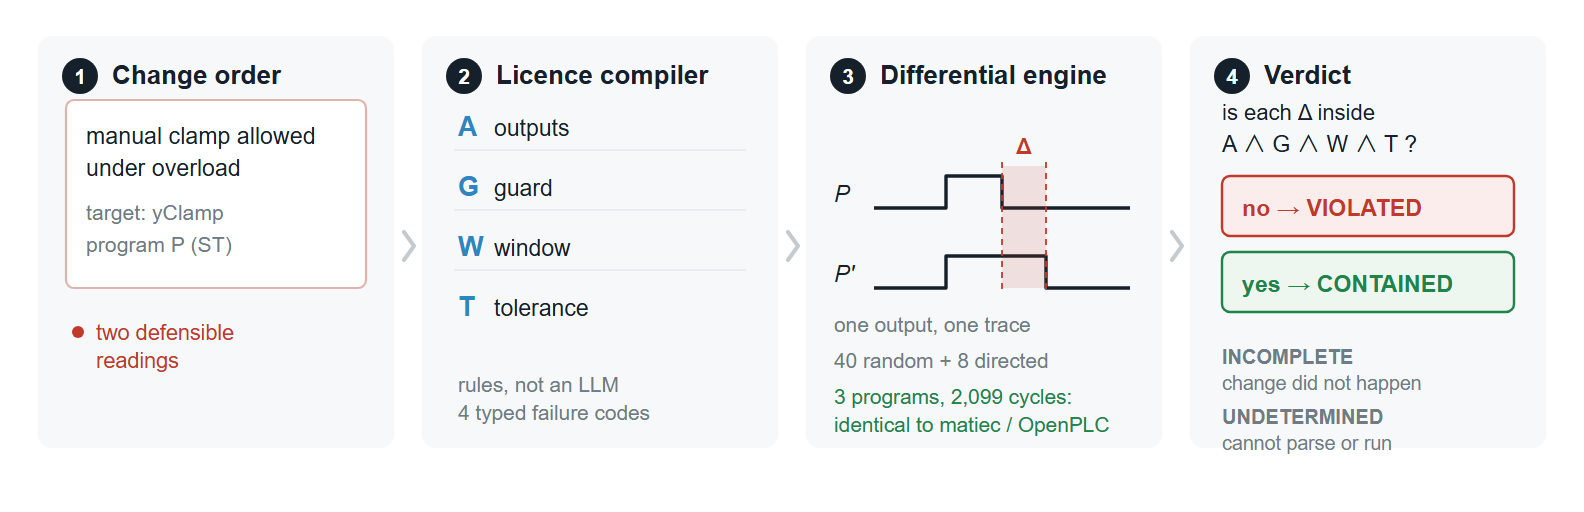
\includegraphics[width=\columnwidth]{figures/fig2_arch.png}
\caption{From an order to a verdict. The order and the program are compiled
into a licence $(A,G,W,T)$ by rules rather than by a model; a cycle-accurate
interpreter runs $P$ and $P'$ on a fixed trace set and records every output
difference; the decision asks whether each difference falls inside the
licensed region. Dashed verticals mark the cycles where the two versions
diverge. \textsc{Incomplete} (a licensed change that did not happen) and
\textsc{Undetermined} (a contract or program the toolchain cannot evaluate)
sit outside the main split.}
\label{fig:pipeline}
\end{figure}

\subsection{Compiling the licence}

Figure~\ref{fig:pipeline} gives the pipeline; the rest of this section takes it stage by stage. The compiler takes the order and the original program and emits one clause $(A,G,W,T)$. It is rule-based, not model-based: a parser extracts the change verb, the target variable, the old and new values, and any condition named in the order, and a rule set fills the four slots. Three decisions are worth stating.

\textbf{Rule-enhanced, not LLM-normalised.} An earlier design normalised paraphrases with an LLM; we dropped it. Rule enhancement reached \textbf{93.8\%} stability over 160 compilations against 34.4\% for unenhanced rules, with the residual 1.25\% concentrated in one mapping (action verb $\to$ input-variable anchor). Dropping the model also keeps the method's failures distinguishable from the model's.

\textbf{Failures are typed, not silent.} Four modes are mapped to codes---\texttt{E\_NO\_TRIGGER}, \texttt{E\_NO\_DELTA}, \texttt{E\_FALLBACK\_G0}, \texttt{E\_AMBIGUOUS}---and a contract that cannot be compiled becomes \textsc{Undetermined} with one of them. It never becomes ``licence everything'', which was the silent-degradation failure of our first implementation.

\textbf{The magnitude bound is derived.} A change from $a$ to $b$ makes behaviour differ for exactly $|b-a|/\mathrm{cycle}$ scans, so the longest contiguous run of differences must lie near that value. The derivation uses only $(C,P)$, never the correct patch, so the bound cannot inherit the answer it checks.

\subsection{The differential engine}

The engine is a cycle-accurate interpreter for a bounded ST subset---no loops, no arrays, single task, \texttt{TON}/\texttt{TOF}/\texttt{R\_TRIG}---that executes $P$ and $P'$ on the same traces and records every output difference as $(t,o,v,v')$.

It is calibrated rather than asserted. Three programs compiled with \textbf{matiec}~\citep{matiec} and run on \textbf{OpenPLC}~\citep{openplc} for \textbf{2,099 cycles} agree \textbf{100\%} on every output and every timer $Q$, including transition points and the first-scan edge of \texttt{R\_TRIG}. One divergence is reported rather than smoothed: after $Q$ is set, matiec/OpenPLC freeze \texttt{TON.ET} at $PT$ while our engine keeps accumulating. IEC 61131-3 leaves this free, and it affects no verdict, because contracts constrain outputs and $ET$ is internal state.

The trace set is fixed and published: \textbf{40 random traces seeded by \texttt{crc32(name)}} plus \textbf{8 directed traces} per program. The seed derives from the program name, so adding a program does not reshuffle the traces of the others. Recall is always reported under this distribution ($\hat{E}$); a recall number without a distribution is not comparable across systems.

\subsection{The requirement bound}

$L(C)$ licenses changes but never requires them, so ``do nothing'' is vacuously contained. $R(C)$ closes that loophole: the change must occur, as a difference inside the licensed region or, for a refactor, as a structural change. Its shape matters more than its presence---an existential bound is blind to under-licensing---so we decompose the region into sub-regions in which the change must be observable, turning $R(C)$ into a conjunction of reachability requirements. Section~\ref{sec:eval} measures what that buys and what it costs.

\subsection{The decision, in one line}

\textsc{Violated} if an unlicensed difference exists, else \textsc{Incomplete} if the requirement is unmet, else \textsc{Contained}, with \textsc{Undetermined} short-circuiting on parse/run failure or an unexpressible contract. This is the most consequential structural fact in the method: the requirement bound can only move \textsc{Contained} to \textsc{Incomplete}, never produce \textsc{Violated}, so it cannot increase detection.

\section{Completeness and Its Bound}
\label{sec:completeness}

\subsection{Two tiers, two duties}

It is tempting to call the two bounds ``orthogonal'' and to claim a two-sided gain. Both claims are false under our implementation, and we say so. \textbf{The upper bound carries all detection}: removing $R(C)$ leaves recall at \textbf{85.4\%, identical}, structurally, because the verdict is \textsc{Violated} if an unlicensed difference exists, else \textsc{Incomplete}, else \textsc{Contained}. \textbf{The lower bound carries rejection and reasons}: it rejects empty patches \textbf{96/96} and unrelated comment/rename patches \textbf{75/80}, adds 12 rejections on positives beyond the upper bound (the 4.9-point gap between recall 85.4\% and rejection rate 90.2\%), and supplies the reason code for under-licensing. An earlier design tested five orthogonality criteria; all five failed and the claim was retired. The division of labour is what remains: the upper bound decides whether a change is inside the licence, the lower bound whether it happened at all.

\subsection{The completeness bound $k$}

The second tier proves absence only up to a bound $k$, and explicit-state enumeration keeps $k$ small. In our pilot, 16 input letters and a 2\,s timer put the required bound at \textbf{220 scans}, where the state space exceeds $10^5$ and the proof does not terminate. So we claim completeness up to $k$ for logic with time constants $\le$ roughly \textbf{20 scans} (interlocks, edge detection, state machines); incompleteness in the \textbf{20--220} band, where the first tier carries the load; and silence beyond it unless the user raises $k$ and pays the cost. ``The two-tier structure is complete'' is false as stated, and we do not claim it.

\subsection{The detector as a reward is exploitable}

Used as a feedback signal, the detector reaches ``compliant'' in 5/5 runs but is \emph{correct} in 0/5: the search moves the change into a corner the contract does not cover. Decomposing $R(C)$ into sub-regions turns the same five samples into \textbf{5/5 compliant and 5/5 correct}, with the trajectory passing through \textsc{Violated} $\to$ \textsc{Incomplete} $\to$ \textsc{Contained}. This is a minimal reproducible form of Goodhart's law, and it bounds what the contribution can be used for: an existential requirement is a target that can be gamed; a decomposed one is a specification a loop can satisfy.

\subsection{What the formalism cannot express}

A restriction order (``toggle only while \texttt{xEn}'') produces its differences exactly in the regime the guard forbids, so the upper bound is structurally blind: it can verify that \emph{some} restriction was implemented, not that the right one was. On our OSCAT probe, four of five verbatim upstream blocks behave like the main corpus, and the fifth (\texttt{TOGGLE} with a newly added interlock) is rejected for this reason. This is a boundary of the formalism, not of the toolchain, and the one place where more engineering does not help: orders that say only what must \textbf{not} happen cannot be checked by containment alone.

\section{Evaluation}
\label{sec:eval}

\subsection{Label semantics: four values, fixed before any number}

Every verdict is one of four values, and the mapping to ``detected / not detected / cannot tell'' was fixed \emph{before} the experiments. \textsc{Violated} (an unlicensed difference exists) is a detection on an over-edit and a false alarm on a control; \textsc{Incomplete} (the upper bound has no objection but a required change did not occur) and \textsc{Contained} (both bounds satisfied) are both correct releases on a control and neither is a detection on an over-edit; \textsc{Undetermined} (parse/run failure, or outside the expressible fragment) is an abstention, reported separately.

We state the mapping because our design document used a \emph{different} three-value set that did not distinguish ``the change was not made'' from ``the change was made and licensed''; reporting the old labels would misattribute \textsc{Incomplete} to detection or abstention depending on the reader. \textsc{Undetermined} is never folded into recall and never counted as an error: folding it either way moves baselines in opposite directions, because a bounded model checker abstains often, so abstention-as-failure penalises it while abstention-as-success rewards a tool that declined to answer. Abstention counts are reported beside every rate.

\subsection{Three units of analysis, and which one carries the claim}

We report every result at three units and never at one alone: a \textbf{point} (a scan index and output where the versions differ), an \textbf{event} (one occurrence of the operating condition the order names), and a \textbf{program/patch} (one $(P,C,P')$ triple, detected if \emph{any} trace exposes an unlicensed difference). The three disagree systematically: sampling outputs every fifth scan costs \textbf{4.9 points} of patch-level recall (80.5\% vs 85.4\%, McNemar $b=12$, $c=0$, exact $p=0.00049$) while being invisible at the ``did it catch the change at all'' level, and a point-level precision of 0.989 in our pilot coexisted with false alarms on 2 of 6 programs. We therefore fix patch-level recall as the primary number, report event-level recall only on the 31 of 96 programs with a countable event, and treat point-level precision as a diagnostic of contract looseness, never as evidence of quality.

\subsection{The input distribution is part of the method, not part of the setup}

A verdict is a function of the programs, the contract \textbf{and the input distribution}. We measure this rather than assume it away: the same detector on the same over-edited patch reports \textbf{40/40} on plant-consistent traces and \textbf{6/40} on unconstrained random traces, because the violation is only observable when consecutive events are separated by more than the hold time---a property of the workload, not of the code. An out-of-distribution trace set costs \textbf{5.7 points} of recall (79.7\% vs 85.4\%), while the environment assumption $\hat{E}$ does not reduce false alarms (0 $\to$ 0); its job is to make the recall denominator well defined. $\hat{E}$ is published as a first-class artifact (generator, fixed seeds, 40 \texttt{crc32(name)} and 8 directed traces per program) and named in every recall claim; a recall number without a distribution is not comparable across systems, and we report none.

\subsection{The verified property is \emph{unlicensed} difference, not difference}
\label{sec:misses}

Formally we check

\begin{equation}
\exists U,\; |U| \le k:\quad \mathrm{Diff}(P,P',U)\setminus L(C)\neq\emptyset
\end{equation}

and not $\mathrm{Diff}\neq\emptyset$. The distinction is not cosmetic. Our first implementation searched for the shortest difference and returned a 6-scan witness that the contract \textbf{licensed} (a timing shift inside the permitted window): the tool reported success while proving nothing about scope. Rewriting the search target as above turned the same witness into evidence.

This definition also determines \textbf{what the 36 misses are}. All 36 have $n_{\mathrm{diffs}}>0$ and $\mathrm{uncovered}=0$: the upper bound was too permissive, not the execution wrong. They fall into two named shapes. \textbf{A, within-tolerance drift} (23): the change moves the right variable by a magnitude inside \texttt{tol} (\eg \texttt{T\#2S} $\to$ \texttt{T\#2020MS}), so every difference is licensed. \textbf{B, guard as the injection surface} (13): the injected difference only manifests when the guard variable is in the licensed state (\eg deleting \texttt{NOT xManual} when the contract licenses changes under \texttt{xManual = TRUE}). No miss is a data defect, so ``85.4\%'' measures a specific property rather than counting bugs.

\subsection{The two bounds do different jobs---and the lower bound does not detect}

Section~4 argued that the lower bound cannot add detection; this is the measurement. Removing $R(C)$ leaves patch-level recall at \textbf{85.4\%---identical}. Its contribution is rejection: empty patches \textbf{96/96}, unrelated comment/rename patches \textbf{75/80}, and 12 extra rejections on positives (the 4.9-point gap between recall 85.4\% and rejection rate 90.2\%), each with an auditable reason code.

\textbf{Shape matters more than presence.} A merely existential $R(C)$ (``some licensed difference occurs'') is blind to under-licensing: \textbf{20 of 123} agent samples (16\%) wrote the window correctly but opened the bypass on an additional condition, licensing only half of what the order granted. We therefore decompose the region: for a bypass order, every input the order leaves unconstrained becomes a sub-region $B\wedge\neg u$ in which the change must also be observable, which turns $R(C)$ into a conjunction of reachability requirements. The effect is measurable in both directions. Offline, five patches that were \textsc{Contained} but differed from the reference become \textsc{Incomplete} with zero unlicensed differences---the verdict now names the defect instead of hiding it. In the loop, those five samples go from 5/5 compliant and \textbf{0/5 correct} to 5/5 compliant and \textbf{5/5 correct}, traversing \textsc{Violated} $\to$ \textsc{Incomplete} $\to$ \textsc{Contained}.

Two limits are stated rather than hidden: the decomposition is a \textbf{sampling approximation} on the trace set, and ``which inputs are unconstrained'' is a judgement---derived here from the correct patch, which would need a human author in deployment. The cost is local: on the 15 affected programs median latency rises \textbf{+42\%} (303 $\to$ 429\,ms); corpus-wide p50 stays at 235\,ms.

\subsection{Stratified reporting and the applicability domain}
\label{sec:layers}

A single corpus-wide number hides the structure of the failure, so we report three layers and fix which one is the headline:

\begin{table}[htbp]
\centering
\small
\setlength{\tabcolsep}{3pt}
\begin{tabular}{@{}p{0.17\columnwidth}p{0.35\columnwidth}p{0.23\columnwidth}p{0.17\columnwidth}@{}}
\toprule
layer & scope & result & role \\
\midrule
\textbf{Claim layer} & orders whose licensed boundary is statically expressible (\texttt{always} / guard / threshold), 65/96 programs & \textbf{155/168 = 92.3\%} & \textbf{headline in the abstract} \\
Full corpus & all 96 programs, 246 observable over-edits & \textbf{210/246 = 85.4\%} (Wilson 80.4--89.2; cluster bootstrap 80.5--90.2) & main RQ1 number in the body \\
Event-window contracts & contracts containing an \texttt{edge} trigger, 31/96 programs & \textbf{55/78 = 70.5\%} & reported separately, never as a headline \\
\bottomrule
\end{tabular}
\caption{Three reporting layers. The headline is the claim layer, not the corpus-wide number. The two numbers in a row have different denominators: 65 (or 31) counts \emph{programs}, 168 (or 78) counts the \emph{over-edit patches} whose orders fall in that layer across those programs; the corpus row has 96 programs and 246 patches.}
\label{tab:layers}
\end{table}

The 21.8-point gap between layers 1 and 3 is \textbf{not} window derivation: all 23 A-shape misses sit in this layer and are tolerance-calibration failures, which answers the natural question ``why not make the window precise?'' with a measurement.

The applicability domain is stated in Section~2.4 as five principles, each fixed before the results; two are load-bearing here. Conditions three and four are the same ones that generated the \textsc{Undetermined} reason codes during the run, and both supporting measurements---the 20--220 scan grey zone and the 31/96 programs with countable trigger edges---predate the main experiment. The domain is therefore a principle and not a post-hoc filter.

\subsection{Setup: what is compared, on what, and how it is scored}

\textbf{Corpus and units.} 96 ST programs, 250 over-edit patches of which 246 are observable (four memory-type programs are reported as an expressibility boundary and excluded from the recall denominator), and 272 control patches: 96 behaviour-preserving edits, 96 empty changes, and 80 unrelated changes. The unit of decision is the patch, not the scan: a patch counts as detected if any trace exposes an unlicensed difference. Aborted runs and out-of-fragment patches are \textsc{Undetermined} and are reported separately, never folded into recall or error.

\textbf{Configurations.} We compare 18 configurations in four groups: six formal\slash differential (three BMC variants with runtime, manual and compiled properties; contract-free diff; manual-contract diff; a SemaDiff-shaped arm~\citep{semadiff}); five static (compile-and-output-set, a manually filled allow table, SDG reachability in two scan variants, and a two-stage LLM static review); six general-model judges (three models $\times$ two prompts, temperature 0, three trials with majority vote); and one reference arm, C7-AI, the C7 engine with an AI-drafted contract. C7-AI is excluded from the main table and from the Holm family because it is not one of the planned configurations.

\textbf{Metrics and tests.} Patch-level recall is \textsc{Violated} over the 246 observable over-edits; FPR is \textsc{Violated} over the 272 controls. Both carry Wilson intervals, and recall a corpus-cluster bootstrap (10,000 resamples, seed 42). Systems are compared on the 506 pairable cases (246 positives + 260 negatives) with exact McNemar, Holm-corrected over the 17 non-reference configurations and, separately, over the eight configurations in the main table---family size is a writing choice, not a property of the data.

\textbf{Two denominators, one mapping.} The 272 controls are 96 behaviour-preserving edits, 96 empty changes, and 80 unrelated changes. Sixteen cases are \texttt{expected\_miss} by construction---four memory-type programs $\times$ four arms---and are excluded from pairing, which leaves \textbf{260 negative cases (92 + 92 + 76)} and \textbf{506 pairable cases (246 positives + 260 negatives)}. The main table reports FPR over all 272; the paired tests use 260. Both are correct and neither is a drift; the mapping is stated here once and repeated in the artifact.

\textbf{What ``correct'' means for a control.} A control patch must not be reported as \textsc{Violated}. \textsc{Contained} and \textsc{Incomplete} both count as a correct release for a control, because neither accuses the patch; for an over-edit, only \textsc{Violated} counts as detected. This asymmetry is deliberate: \textsc{Incomplete} says ``the required change did not happen'', which is a rejection of the patch, not a scope accusation.

We do \textbf{not} claim higher balanced accuracy than an LLM judge: our own comparison puts the strongest judge at 97.0\% against our 92.9\% on the 506-case set. What we claim is a zero-false-alarm operating point, determinism, auditability, and a measured account of where and why the approach fails.

\subsection{RQ1 --- Under a zero-false-alarm constraint, how much does a compiled licence detect?}

\textbf{Answer: 210/246 = 85.4\% corpus-wide, 155/168 = 92.3\% on the statically expressible layer, with 0/272 false alarms} (Wilson upper bound 1.39\%), at 235\,ms p50 per case and zero API cost.

The two numbers are not interchangeable. The 92.3\% layer contains the 65 programs whose licensed boundary is statically expressible; it is the layer the method claims. The 85.4\% number is the complete measurement over all 96 programs and is what we put in the body. Event-window programs account for the gap: 55/78 = 70.5\%, reported separately and not claimed. The 36 misses are analysed in Section~\ref{sec:misses}: all have an over-permissive upper bound, and none is a data defect.

\textbf{Why this is the right headline for a zero-FPR tool.} A false alarm in change review is not a harmless extra check: it blocks a work order and consumes an engineer's review slot. The design therefore fixes FPR at zero and asks how much recall is available at that point. Section~\ref{sec:rq2} shows that this is also where the method sits on the empirical Pareto frontier---and that the frontier is short.

\subsection{RQ2 --- Where does the method sit among 18 configurations, and when is it the right choice?}
\label{sec:rq2}

We answer in three steps: the full table, the Pareto frontier, and the cost boundary that decides between the frontier points.

\subsubsection{The main table}

\begin{table}[htbp]
\centering
\scriptsize
\setlength{\tabcolsep}{3.2pt}
\begin{tabular}{@{}l l r r r r r r@{}}
\toprule
configuration & grp & recall & FPR & acc. & $b/c$ & $p$ & $p_{\mathrm{Holm}}$ \\
\midrule
\textbf{ours} & --- & \textbf{85.4} & \textbf{0.0} & 92.9 & --- & --- & --- \\
C3 BMC runtime & F & 0.0 & 0.0 & 38.7 & 101/0 & $7.9\mathrm{e}{-31}$ & $6.3\mathrm{e}{-30}$ \\
C4 BMC + manual props & F & 68.3 & 2.9 & 84.8 & 39/0 & $3.6\mathrm{e}{-12}$ & $2.2\mathrm{e}{-11}$ \\
C5 BMC + compiled props & F & 68.3 & 0.7 & 84.4 & 43/0 & $2.3\mathrm{e}{-13}$ & $1.6\mathrm{e}{-12}$ \\
C6 diff, no contract & F & 100.0 & 31.6 & 83.8 & 82/36 & $2.8\mathrm{e}{-05}$ & $1.1\mathrm{e}{-04}$ \\
C7 diff + manual contract & F & 68.7 & 2.2 & 89.1 & 21/0 & $9.5\mathrm{e}{-07}$ & $4.8\mathrm{e}{-06}$ \\
C-SD SemaDiff-shaped & F & 98.8 & 30.5 & 83.8 & 82/36 & $2.8\mathrm{e}{-05}$ & $8.3\mathrm{e}{-05}$ \\
C-LS two-stage static & S & 99.6 & 8.5 & 95.2 & 24/36 & $1.6\mathrm{e}{-01}$ & $1.6\mathrm{e}{-01}$ \\
L5-Qwen line-by-line & L & 100.0 & 5.5 & 97.0 & 15/36 & $4.6\mathrm{e}{-03}$ & $9.2\mathrm{e}{-03}$ \\
\textit{C7-AI (reference)} & R & \textit{98.8} & \textit{5.1} & \textit{96.8} & \textit{13/33} & \textit{$4.5\mathrm{e}{-03}$} & --- \\
\bottomrule
\end{tabular}
\caption{Main comparison. Recall is over 246 observable over-edits, FPR over 272 controls, accuracy over the 506 pairable cases. $b/c$ is exact McNemar against ours; the Holm family has 8 members (the 17-configuration family is in the artifact). Groups: F formal/differential, S static, L LLM judge, R reference arm.}
\label{tab:main}
\end{table}

Two rows run against the narrative. \textbf{L5-Qwen and C7-AI have higher balanced accuracy than our method} (97.0\% and 96.8\% vs 92.9\%), significant after Holm for L5-Qwen ($9.2\mathrm{e}{-03}$) and uncorrected for C7-AI ($4.5\mathrm{e}{-03}$). Both pay for it in false alarms: 5.5\% and 5.1\% FPR, \ie 53 and 49 per 1,000 changes at a 4.3\% prevalence.

\subsubsection{The frontier has three points}

Plotting all 18 configurations on (FPR, recall) leaves three non-dominated points: ours (0\%, 85.4\%), C7-AI (5.1\%, 98.8\%), L5-Qwen (5.5\%, 100\%). Everything else is dominated, including the three contract-bearing formal/differential configurations---C4 (2.9\%, 68.3\%), C5 (0.7\%, 68.3\%), C7 (2.2\%, 68.7\%)---which are worse than ours on \textbf{both} axes; C6 and C-SD buy recall only with a 30\% false-alarm rate. The frontier is a staircase with two steps, and no configuration reaches 95\% recall at 1\% FPR. That absence is itself a finding: the mechanisms that buy recall also release false alarms, so the trade-off is not smooth (Figure~\ref{fig:workpoint}).

\begin{figure}[htbp]
\centering
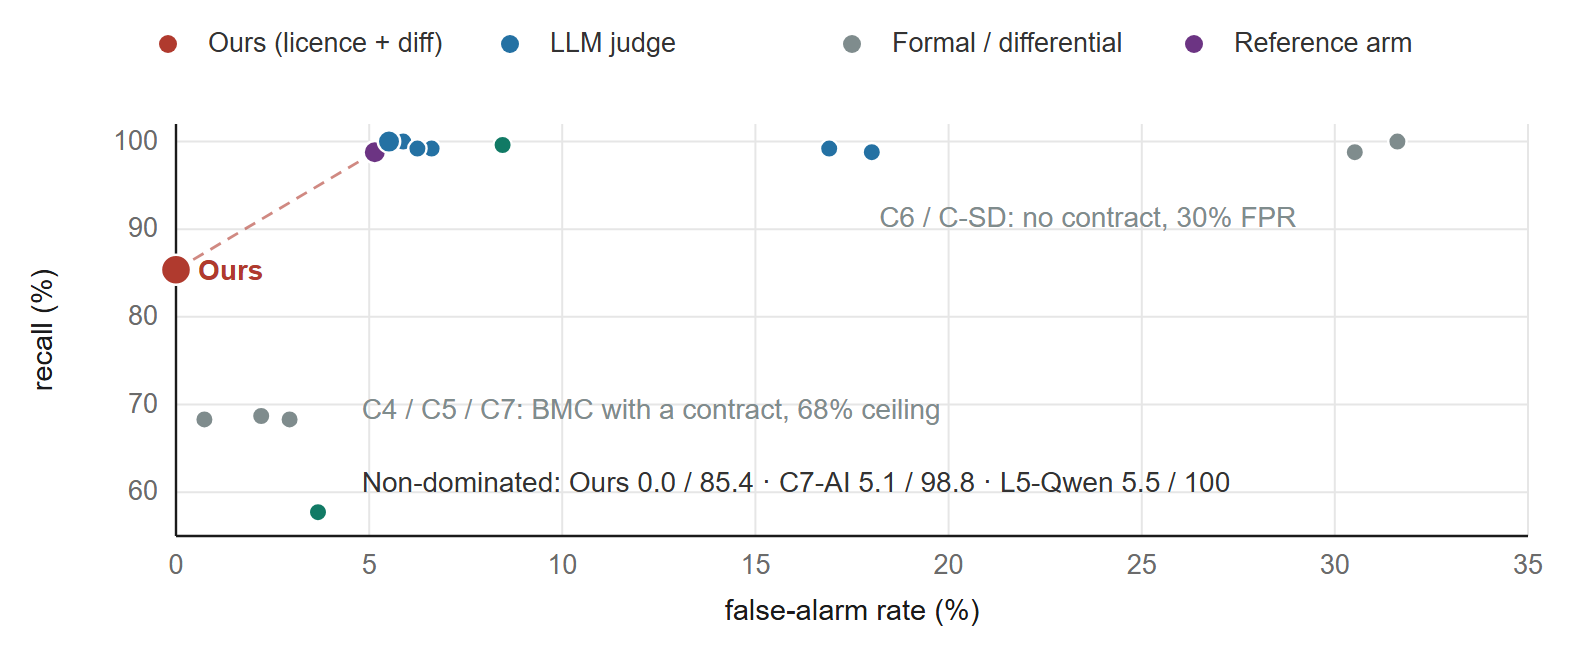
\includegraphics[width=\columnwidth]{figures/workpoint.png}
\caption{Recall against false-alarm rate over 522 cases, one point per configuration. Colour gives the family; the dashed line links the three non-dominated points. The two bounded-model-checking configurations with a contract (C4, C5) activate only 59 and 44 of the 96 order entries and both stop at 68.3\% recall, while the manual-contract diff (C7) reaches 68.7\%; C6 and C-SD reach $\sim$99\% only by accepting a 30\% false-alarm rate.}
\label{fig:workpoint}
\end{figure}

\subsubsection{The cost boundary}

Whether the 5\% step is worth taking is a cost question, not an accuracy question. With cost $=\mathrm{FP}\cdot c_{\mathrm{FP}}+\mathrm{FN}\cdot c_{\mathrm{FN}}$ per 1,000 changes at $\pi=4.3\%$:

\begin{table}[htbp]
\centering
\small
\begin{tabular}{@{}l r r l@{}}
\toprule
alternative & extra FP / 1{,}000 & fewer FN / 1{,}000 & alternative better iff \\
\midrule
L5-Qwen line-by-line & 52.8 & 6.3 & $c_{\mathrm{FN}}/c_{\mathrm{FP}} > \mathbf{8.39}$ \\
C7-AI & 49.3 & 5.8 & $c_{\mathrm{FN}}/c_{\mathrm{FP}} > \mathbf{8.54}$ \\
C-LS & 80.9 & 6.1 & $c_{\mathrm{FN}}/c_{\mathrm{FP}} > \mathbf{13.23}$ \\
C6 & 302.6 & 6.3 & $c_{\mathrm{FN}}/c_{\mathrm{FP}} > \mathbf{48.08}$ \\
\bottomrule
\end{tabular}
\caption{Cost boundary at 4.3\% prevalence. Below the threshold, ours is cheaper.}
\label{tab:cost}
\end{table}

The method is therefore the better choice whenever a missed over-edit costs less than 8.4 times a false alarm. That is defensible in work-order review---a false alarm costs a review slot and a blocked order, a miss can still be caught by the next gate---but it is an assumption, and we state it as one: when misses are catastrophic and review capacity is abundant, the 5\% step is rational (Figure~\ref{fig:cost}).

\begin{figure}[htbp]
\centering
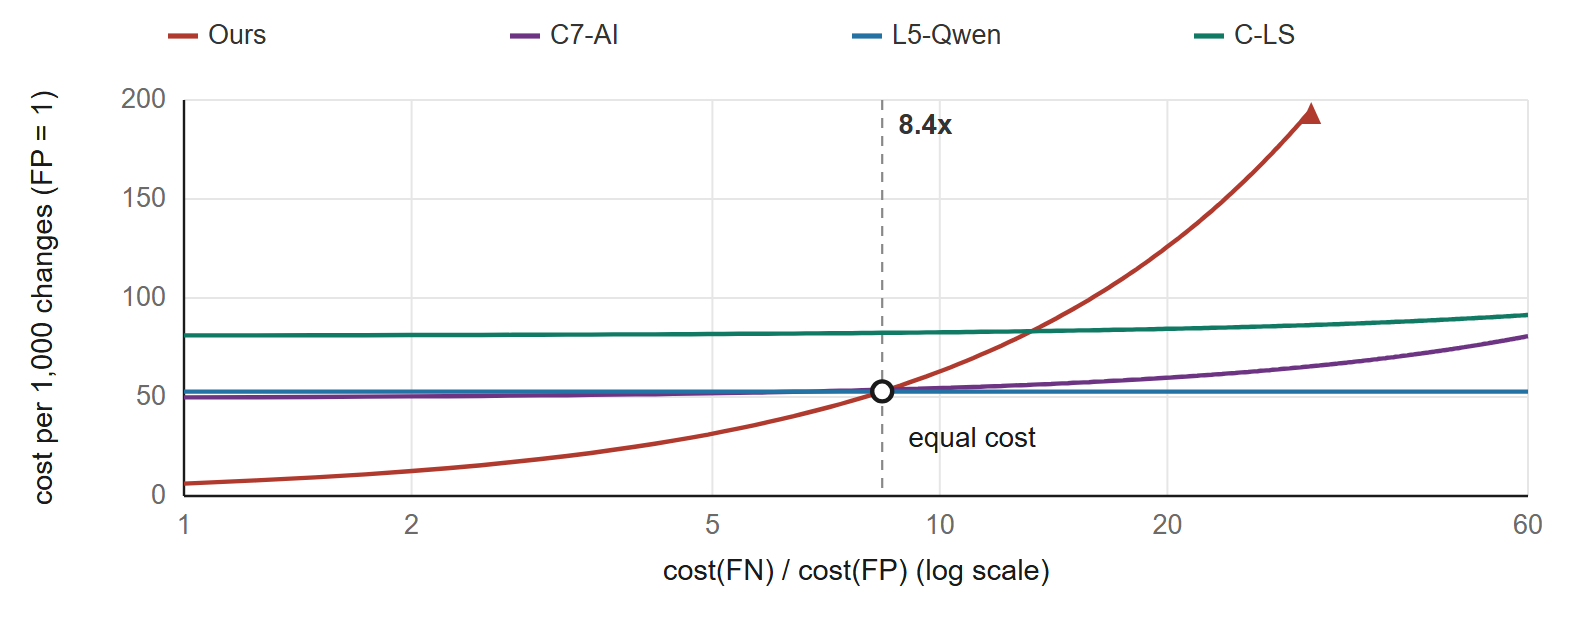
\includegraphics[width=\columnwidth]{figures/cost_curve.png}
\caption{Cost per 1,000 changes against the ratio of miss cost to false-alarm cost, at 4.3\% prevalence. The near-flat curves are high-recall configurations paying a constant false-alarm bill; ours starts near zero and rises with the ratio. The two curves cross at $c_{\mathrm{FN}}/c_{\mathrm{FP}}=8.4\times$; below it our method is cheaper. The axis stops at 200, so our curve leaves the panel through the arrow at roughly $32\times$ and is not flat.}
\label{fig:cost}
\end{figure}

\subsubsection{Prevalence matters more than the balanced set}

The 506-case set is balanced by construction; deployment prevalence is not. At $\pi=4.3\%$ (the exploratory rate from the T3 sample) precision is 100\% for ours and 44.9\% for L5-Qwen---0 and 53 false alarms per 1,000 changes. Figure~\ref{fig:pi} plots precision against $\pi$ for the five main configurations: our curve is flat at 100\%, while the judges converge to it only as $\pi\to 1$. This is the comparison that matters for a review pipeline, and we report it beside the balanced-set table, not instead of it.

\begin{figure}[htbp]
\centering
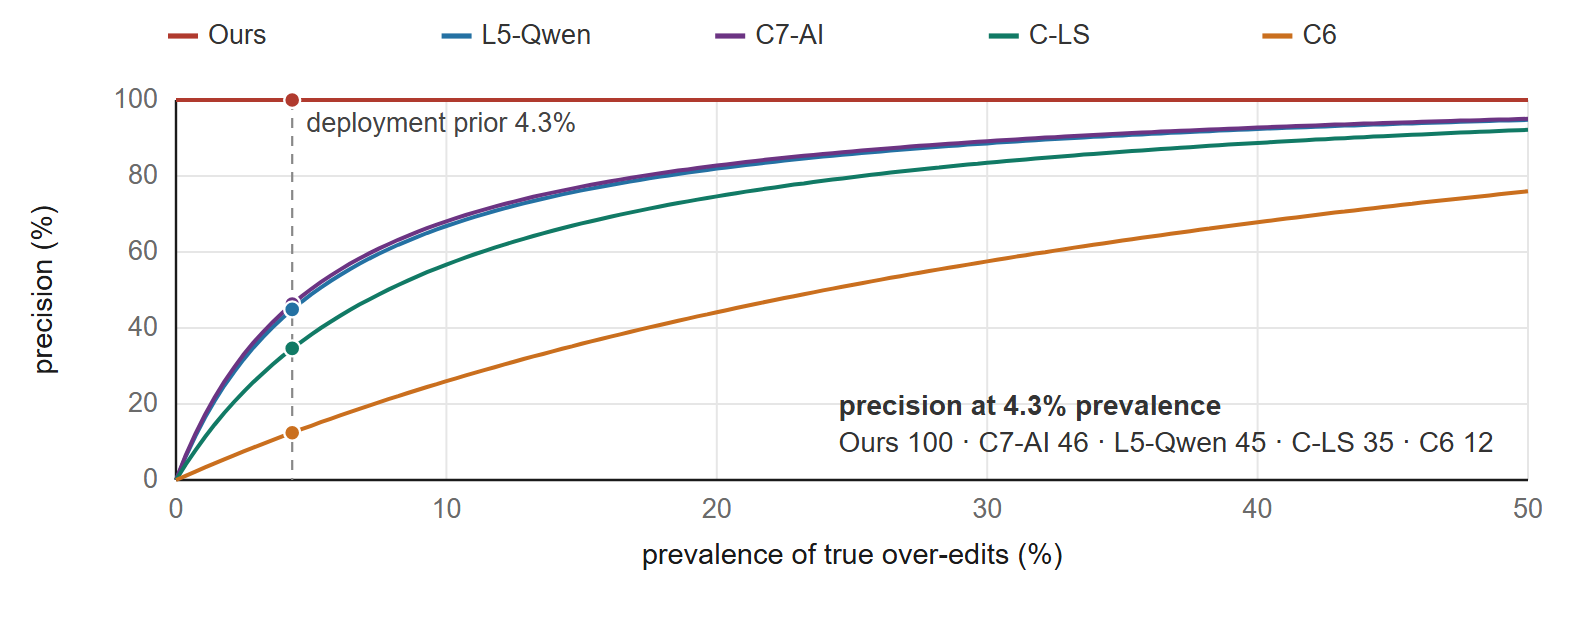
\includegraphics[width=\columnwidth]{figures/pi_curve.png}
\caption{Precision as a function of the prevalence of true over-edits. Dots mark the T3 rate of 4.3\%: 100\% for ours against 46\% (C7-AI), 45\% (L5-Qwen), 35\% (C-LS) and 12\% (C6). Our curve is flat because it raises no false alarms; every other curve rises only as prevalence approaches one.}
\label{fig:pi}
\end{figure}

\subsection{RQ3 --- What moves the work point: the engine or the contract?}

Five controlled contrasts point to contract tightness, not the engine.

\textbf{Contract on/off, same engine.} C6 (no contract) is 100\% / 31.6\%; C7 (manual contract) 68.7\% / 2.2\%: the contract removes 93\% of the false alarms and costs 31 points of recall.

\textbf{Who writes the contract, same engine.} C7 is 68.7\% / 2.2\%; C7-AI is 98.8\% / 5.1\%. Same engine, traces and corpus; only the contract source changes. The AI contract is tighter---fewer licensed outputs on 35 of 96 entries (45 identical, 16 looser), mean licensed-output count 1.73 against 2.08, a window on 31 entries against 15, and a narrower window on 13 of the 15 shared entries. Tighter licence, more differences outside it: higher recall and higher FPR. This is the cleanest evidence that the work point is a contract property.

\textbf{Property source under the same BMC engine.} C4 is 68.3\% / 2.9\%; C5 is 68.3\% / 0.7\%: recall identical, only false alarms move.

\textbf{BMC versus differential execution.} C4/C5 (68.3\%) against ours (85.4\%): the gap is engine coverage, not the contract---C4 has 32 \textsc{Undetermined} (29 \texttt{NO\_PROPERTY}, 3 timeout), C5 21 (16, 5), C3 331 (195 timeout, 132 front-end rejection). A checker that cannot discharge the property cannot detect the change, however tight the contract.

\textbf{Trace generator.} C6 is 100\% / 31.6\%; C-SD is 98.8\% / 30.5\%: 1.2 points of recall and 1.1 of FPR. The stimulus is not the lever.

The contracts themselves show the same ordering:

\begin{table}[htbp]
\centering
\small
\begin{tabular}{@{}l r r r r r@{}}
\toprule
configuration & active & mean allowed & windows & mean width & $\mathrm{tol}>0$ \\
\midrule
ours & 86/96 & 2.27 & 0 & --- & 0 \\
C4 (manual props) & 59/96 & 1.41 & 15 (15.6\%) & 197.8 & 0 \\
C5 (compiled props) & 44/96 & 1.52 & 31 (32.3\%) & 375.3 & 0 \\
C7 (manual contract) & 86/96 & 2.08 & 15 (15.6\%) & 197.8 & 0 \\
C7-AI (AI contract) & 86/96 & 1.73 & 31 (32.3\%) & 213.7 & 1 \\
\bottomrule
\end{tabular}
\caption{Contract tightness: activated entries, mean licensed outputs among active entries, window coverage and width, and entries with a positive tolerance.}
\label{tab:tight}
\end{table}

Two quantities explain most of the variance. \textbf{Activation rate} separates the BMC configurations: C4 activates 59/96 entries and C5 44/96, so more than a third of the corpus is \textsc{Undetermined} before any judgement is made; that is the 68\% ceiling. \textbf{Licensed-output width} separates the contract sources at the same activation rate: 2.27 (ours) $>$ 2.08 (C7) $>$ 1.73 (C7-AI), exactly the order of FPR (0 $<$ 2.2 $<$ 5.1). Recall is not monotone in width alone: C7 sits at 68.7\% because it enables a window on only 15 entries, whereas C7-AI enables 31 and reaches 98.8\%. Recall therefore follows the \emph{joint} tightness of allow width and window coverage, not either one alone. The work point is not a property of the model or the solver; it is a property of how wide a licence the contract draws.

\subsection{RQ4 --- Is order clarity a larger lever than the detector?}

\textbf{Yes, and it is upstream of every configuration in Section~\ref{sec:rq2}.} Holding program, model and compiled contract fixed and rewriting only the wording moves the violation rate from \textbf{6/6 to 0/10} with byte-identical patches; the residual failure has a nameable shape (bypass-key substitution) across two model families, and under clear orders the dominant error reverses: \textbf{20 of 123} samples (16\%) under-license. No detector can fix this---a judge reads the same ambiguous order, a compiler parses the same text, a BMC is given the same property---so a pipeline that invests in detectors but not in order templates optimises the wrong stage.

\subsection{What the evaluation establishes, and what it does not}

\textbf{Establishes}: a zero-false-alarm operating point at 85.4\% recall (92.3\% on the claim layer), reproducible from a fixed trace set at zero API cost; a three-point Pareto frontier over 18 configurations with a cost boundary at $c_{\mathrm{FN}}/c_{\mathrm{FP}}=8.4\times$; a mechanism---the work point is set by contract tightness, not by the engine or the model; and one upstream failure mode, order clarity, that moves the violation rate from 6/6 to 0/10 independently of the detector.

\textbf{Does not establish} superior balanced accuracy: L5-Qwen is better on the 506-case set (97.0\% vs 92.9\%, Holm $p=9.2\mathrm{e}{-03}$), and the abstract does not claim otherwise. Nor an independent human baseline: both annotation sets have one AI-assisted annotator, so L6 (26/30) is a single-reviewer reference point. The C5 and C7 acceptance caveats are stated in Section~\ref{sec:threats}.

\section{Threats to Validity}
\label{sec:threats}

\subsection{Construct validity}

\textbf{Change orders are authored by us.} A synthetic order is cleaner than a real one, which inflates compilation quality and understates ambiguity. \emph{Mitigation}: an agent-generated layer under the same orders (395 samples, two model families) and a measured clarity study---holding program, model and compiled contract fixed, only the wording changes, violation rate 6/6 $\to$ 0/10 with byte-identical patches. This turns the threat into a finding without removing it: the orders are still not written by plant engineers. The opening scenario is a composite of prior failure reports and our interviews, and the paper says so where it appears.

\textbf{``Licensed delta'' is defined by the reference change.} If the reference is wrong, the contract is wrong in the same direction. \emph{Mitigation}: several independent correct implementations per program, with the contract-to-implementation gap reported.

\textbf{Prevalence is not a population estimate.} Among 395 agent samples, 8 are clean true violations across four orders ($\approx$2\%) and 9 more are ambiguous orders reported separately; we claim detection capability (8/8) and the dependence on clarity, not a population rate.

\textbf{The human annotations are single-annotator and AI-assisted.} The A1 allow table (96 rows) and the L6 sample (30 cases) each have one annotator, both AI-assisted, so no two-person $\kappa$ exists. L6 scores 26/30 (20/22 recall, 2/8 FPR); we report it as a single-reviewer reference point, not an expert blind baseline.

\textbf{The interviews are formative, and two participants are not a sample.} Two engineers at two plants, recruited through a project partner, cannot support claims about prevalence or preference. They serve two narrow purposes---confirming that the first question a reviewer asks concerns the object of change, and finding which parts of the four-tuple need explanation---and the checklist they produced is justified by the experiment (6/6 $\to$ 0/10), not by the interviews.

\textbf{Contract legibility is confounded by our own stimulus.} The card lists all four fields, so both engineers could paraphrase \texttt{allow}, \texttt{guard}, \texttt{window} and \texttt{tol}: that is reading comprehension of our artifact, not evidence that the notation is usable. What carries information is where they failed---neither could convert \texttt{cycles} to time without the scan period---and what they asked for: the order sentence, the program location, the approver, and the before/after values.

\subsection{Internal validity}

\textbf{Our interpreter is not a conformant IEC 61131-3 runtime.} It supports a bounded subset (no loops, no arrays, single task, \texttt{TON/TOF/R\_TRIG}), and integer division, implicit conversion and scheduling may differ from vendor toolchains. \emph{Mitigation}: three programs compiled with \textbf{matiec} and run on \textbf{OpenPLC} for \textbf{2,099 cycles} agree \textbf{100\%} on every output and every timer $Q$, including transition points and the first-scan edge of \texttt{R\_TRIG}. One divergence is reported rather than smoothed: after $Q$ is set, matiec/OpenPLC freezes \texttt{TON.ET} at $PT$ while our engine keeps accumulating. IEC 61131-3 leaves this free, it affects no verdict (contracts constrain outputs, $ET$ is internal state), and we leave the engine unchanged---changing it would invalidate 250 patches, 522 cases and 395 historical samples.

\textbf{Determinism is asserted, not assumed.} Fixed seeds; two runs must give bit-identical verdicts with only wall-clock varying. A non-deterministic judge is the failure mode we criticise.

\textbf{The delivered C5 properties required normalisation.} Of the 96 YAML files our compiler produced, 44 had serialization defects: 30 wrote \texttt{guard} with quotes, which the receiving group's reader treated as part of the value and turned into a vacuously true assertion (a \textbf{silent false negative}); 10 used a shape-invalid \texttt{kind} that nevertheless generates a byte-identical harness; 4 lacked a top-level \texttt{reason}. The group repaired the reader and normalised the files before execution, so the C5 numbers describe \textbf{delivered properties after documented normalisation}, not as-delivered behaviour, and the executed set is not in the package.

\textbf{Nine of 522 cases differ by one line between local and delivered versions.} Three guard programs exist in two versions differing by an \texttt{AND xPermit} clause. We checked all nine affected cases against four configurations: six positives are \textsc{Violated} and three negatives \textsc{Contained} in every configuration---\textbf{zero verdicts flip}. The artifact must ship one version; the reported numbers do not depend on which.

\subsection{External validity}

\textbf{Corpus provenance is skewed to self-built programs.} Of 96 programs, \textbf{9 are upstream-derived and 87 self-built}---an upstream-backed share of \textbf{9\%}. OSCAT Basic is the backbone (173 function blocks, 82 directly expressible in our subset, 42 more with \texttt{CASE}/\texttt{FOR}), but the programs carrying our orders are minimal constructions isolating one mechanism each. External validity is argued by \emph{mechanism}, not by scale, and this is the weakest link in the paper.

\textbf{A verbatim-upstream probe bounds the ``written for the method'' objection.} Five OSCAT~\citep{oscat} blocks were ported verbatim through the identical pipeline. Four behave like the main corpus: on \texttt{SEL2\_OF\_3B} the contract recovers the exact output set and magnitude bound (50 scans for 500 $\to$ 1000\,ms), catching 5 of 6 over-edits; on \texttt{DRIVER\_1} the bound is 150 scans for 500\,ms $\to$ 2\,s and both are caught; on \texttt{INTERLOCK} the bound is 50 scans and both are caught, after fixing a \texttt{TOF} falling-edge defect the main corpus could not expose. The fifth (\texttt{TOGGLE} with a newly added interlock) is rejected for a formal reason (Section~4.4).

\textbf{Corpus shape, language and toolchain.} C-class programs are 15--25 lines; plant-scale state spaces are untested; four programs fall outside the expressible fragment; only Structured Text is covered, with Ladder and FBD out of scope. No vendor IDE is exercised, a single 10\,ms cycle and single-task execution are assumed, and multi-task priority and jitter are not modelled.

\subsection{Conclusion and statistical validity}

The $k$-bound of Section~4.2 is the conclusion-validity boundary: beyond roughly 220 scans we claim nothing. Patches from the same program are not independent, so we cluster-bootstrap by program (10,000 resamples, seed 42) and report Wilson intervals only where case-level independence holds; the 85.4\% estimate carries a cluster interval of 80.5--90.2\%, wider than the Wilson interval (80.4--89.2\%), and the abstract uses the wider one. Seventeen non-reference configurations are compared, so Holm-adjusted values are reported for that family and for the eight configurations in the main table, because family size is a writing choice. Abstention is uneven---C4 has 32 \textsc{Undetermined}, C5 21, and C3 only 191 evaluable cases---so every rate carries its denominator and no 191-case rate is compared with a 506-case rate without saying so.

Four claims from earlier drafts are retired: C7's 150/145 acceptance counts (no window convention reproduces them; the released configuration is \textbf{179/285/58}, and the 13 boundary differences flip zero verdicts); superior balanced accuracy (97.0\% and 96.8\% against our 92.9\%); an independent expert baseline (both annotators single and AI-assisted); and C5 ``as delivered'' (the executed set is normalised and absent from the package).

\section{Discussion}
\label{sec:discussion}

\subsection{Three findings that outlive the tool}

\textbf{The lower bound does not detect, and that is the point.} Removing the requirement bound leaves recall unchanged, because the verdict structure only allows \textsc{Contained} $\to$ \textsc{Incomplete}. Its job is to reject patches that did not do the job (96/96 empty, 75/80 unrelated) and to name under-licensing. A reader expecting a two-sided contract to improve detection will be surprised; the surprise is the finding, and it means a pipeline should budget the two bounds separately.

\textbf{Over-edit rate is a function of order clarity, not of the model.} Holding program, model and contract fixed, the 6/6 $\to$ 0/10 shift with byte-identical patches says the input, not the agent, is the dominant variable; the residual failure has a stable shape (bypass-key substitution) across model families. Order templates and disambiguation checklists may therefore buy more than another detector.

The interviews give the human shape of the same gap. Both engineers named the object first---``which variable, which timer, there are three startup delays on that line''---and then, asked which of the four items actually causes trouble, switched to the boundary: ``eight of ten unclear orders are unclear about the object. But what I most want written down is what must not be touched\ldots{} A wrong object wastes time; a wrong boundary causes accidents.'' The other supplied the rework: while changing a delay, an alarm output was edited along with it, caught only at the trial run. Checklists follow the order questions are asked, but the field cost sits in the item asked last, which is why our template makes ``must not change'' a required field checked first.

Both also failed the same way on notation rather than on logic: neither could turn a window written in scans into a time without being told the scan period, so the same clause denotes 500\,ms on a 10\,ms cycle and 2\,s on a 40\,ms one. That is a four-fold different boundary drawn by the same sentence, and it is why the contract display carries both units and why the order template asks for the period explicitly.

\textbf{Event-window contracts are worse for a nameable reason.} The 70.5\% on edge contracts is not a window-derivation failure; all 23 A-shape misses are within-tolerance drift, because the contract carries a magnitude tolerance. The target is tolerance calibration, a different project from making the window precise.

\subsection{Using, and designing for, a work point}

A detector of this kind is a \emph{gate}, not a judge: it can block a change outside the licensed region and attach a reason code a human can audit, but it cannot say whether a change is \emph{good}, only whether it is in scope. The human signature remains the authority.

The zero-false-alarm point is a deliberate operating choice, not a claim of superiority. Where a false alarm costs a review slot and a blocked order, the 8.4$\times$ boundary is a reasonable default; where a miss is catastrophic and reviewers are abundant, the judge's 5\% step is rational. We state the boundary so the choice is explicit rather than inherited from a benchmark rank.

The 18-configuration study suggests the first design decision is not the engine but the \emph{licence width}: activation rate sets the ceiling of what can be checked (44--59 of 96 entries for the BMC configurations), and licensed-output width sets the false-alarm rate at a fixed activation rate (2.27 $\to$ 0\%, 2.08 $\to$ 2.2\%, 1.73 $\to$ 5.1\%). A single (recall, FPR) point hides that choice; a work-point report lets a reader place the tool in their own cost structure.

The strongest LLM judge is not a straw man---97.0\% balanced accuracy against our 92.9\%, and simpler to deploy. The difference is the artefact: a judge returns a verdict and a rationale, not a licence a human can read, diff, version and reuse. The two are complementary, and the C7-AI arm shows the boundary is movable, which is why the contract, not the engine, is the design variable.

\section{Related Work}
\label{sec:related}

Four tool families are routinely applied to a PLC change. Each answers a different question, and none asks ours---\emph{should this change have happened here?}

\subsection{Behavioural diffing and regression testing}

Differential testing and regression-test selection compare versions by behaviour. They answer \emph{did behaviour change}; we answer \emph{was this change permitted}, and treat behavioural equality as a reason to stop looking rather than as a verdict. Change-distilling techniques recover fine-grained edit operations from syntax trees \citep{changedistiller} and the complementary problem, deciding from generated tests whether a commit preserved behaviour at all, is now attacked directly~\citep{semadiff}; both still answer \emph{did behaviour change}, which is why a change that is correctly detected as behaviour-changing says nothing about whether it was allowed.

\subsection{Formal verification for PLC}

Bounded model checking reaches PLC code through CBMC and ESBMC \citep{cbmc,esbmc}, and PLCverif integrates it into industrial workflows \citep{plcverif}. These engines answer \emph{is the code correct with respect to a specification}, and they are reliable; the bottleneck is that someone must write the specification. We compile it from the work order. Our C4/C5 contrast measures exactly this: on the same engine, hand-written and compiled properties give identical recall (68.3\%) and differ only in false alarms (2.9\% vs 0.7\%), so the property source buys precision, not detection.

\subsection{Static analysis and rule-based review}

Static rule mining and pattern-based review answer \emph{does the change match rules extracted from history}. They scale without execution, and they cannot see timing- or window-shaped over-edits: a timer moved by 20\,ms leaves every syntactic rule satisfied. Our C1a/C2/C-LS configurations measure the family; its strongest member reaches high recall only with an 8.5\% false-alarm rate, and its precise members (C1b, C2) have low recall.

\subsection{LLM-based review and coding agents}

LLM review and repair agents answer \emph{does it look right}: they have improved rapidly \citep{codereviewer,swebench}, and recent work documents that they often make unrequested edits \citep{logrem}. Our L5 configurations instantiate the family across three models and two prompts. The finding is not that LLMs are bad at the task---they reach 97--100\% recall---but that without a licence they buy recall with false alarms, and their verdicts are not reproducible at the level a review process requires (three-trial agreement 88.9--97.5\%).

\subsection{PLC change management and IEC 61131-3}

PLC programs are governed by IEC 61131-3 \citep{iec61131}, and industrial change management is organised around work orders, version control and sign-off. The work order is a natural-language artefact read by humans and, until now, not executable. We make it executable as a licence while keeping it readable: $(A,G,W,T)$ is small enough for an engineer to audit and precise enough for a differential engine to enforce. What we judge is containment in that licence---not correctness, not style, and not whether the change was written well.

\section*{Data Availability}\label{sec:data}

An anonymised artifact accompanies this submission as anonymous supplementary
material. It contains the 96-program corpus (for each program: the change
order, the pre-change program, the reference implementation and the injected
over-edits), the $522\times18$ verdict matrix, the licence compiler, the
evaluation scripts and the sources of all five figures. Running
\texttt{python reproduce.py --full} recomputes every number in
Section~\ref{sec:eval} in about four minutes, and exits non-zero if any value
moves; it needs no network access and no third-party package. A public
repository with a permanent identifier will be linked from the camera-ready.

\bibliographystyle{ACM-Reference-Format}
\bibliography{refs}

\end{document}
